\documentclass[12pt]{standalone}

\usepackage{bm}
\usepackage{tikz}
    \usetikzlibrary{arrows.meta}

\def \D { 
	0/0 , 5/0 , 10/0 , 15/0 , 20/0 , 
	4/2 , 
	1/3 , 11/3 , 16/3 , 21/3 , 
	3/4 , 
	15/5 , 20/5 , 2/6 , 12/6 , 1/8 , 6/8 , 16/8 , 21/8 , 3/9 , 13/9 , 0/10 , 5/10 , 20/10 ,  7/11 , 12/11 , 17/11 , 4/12 , 19/12 , 24/12 , 11/13 , 21/13 , 3/14 , 8/14 , 18/14 , 23/14 , 12/16 , 22/16 , 4/17 , 9/17 , 21/18 , 3/19 , 8/19 , 13/19 , 23/19 , 20/20 , 4/22 , 9/22 , 14/22 , 19/22 , 24/22 }


\begin{document}
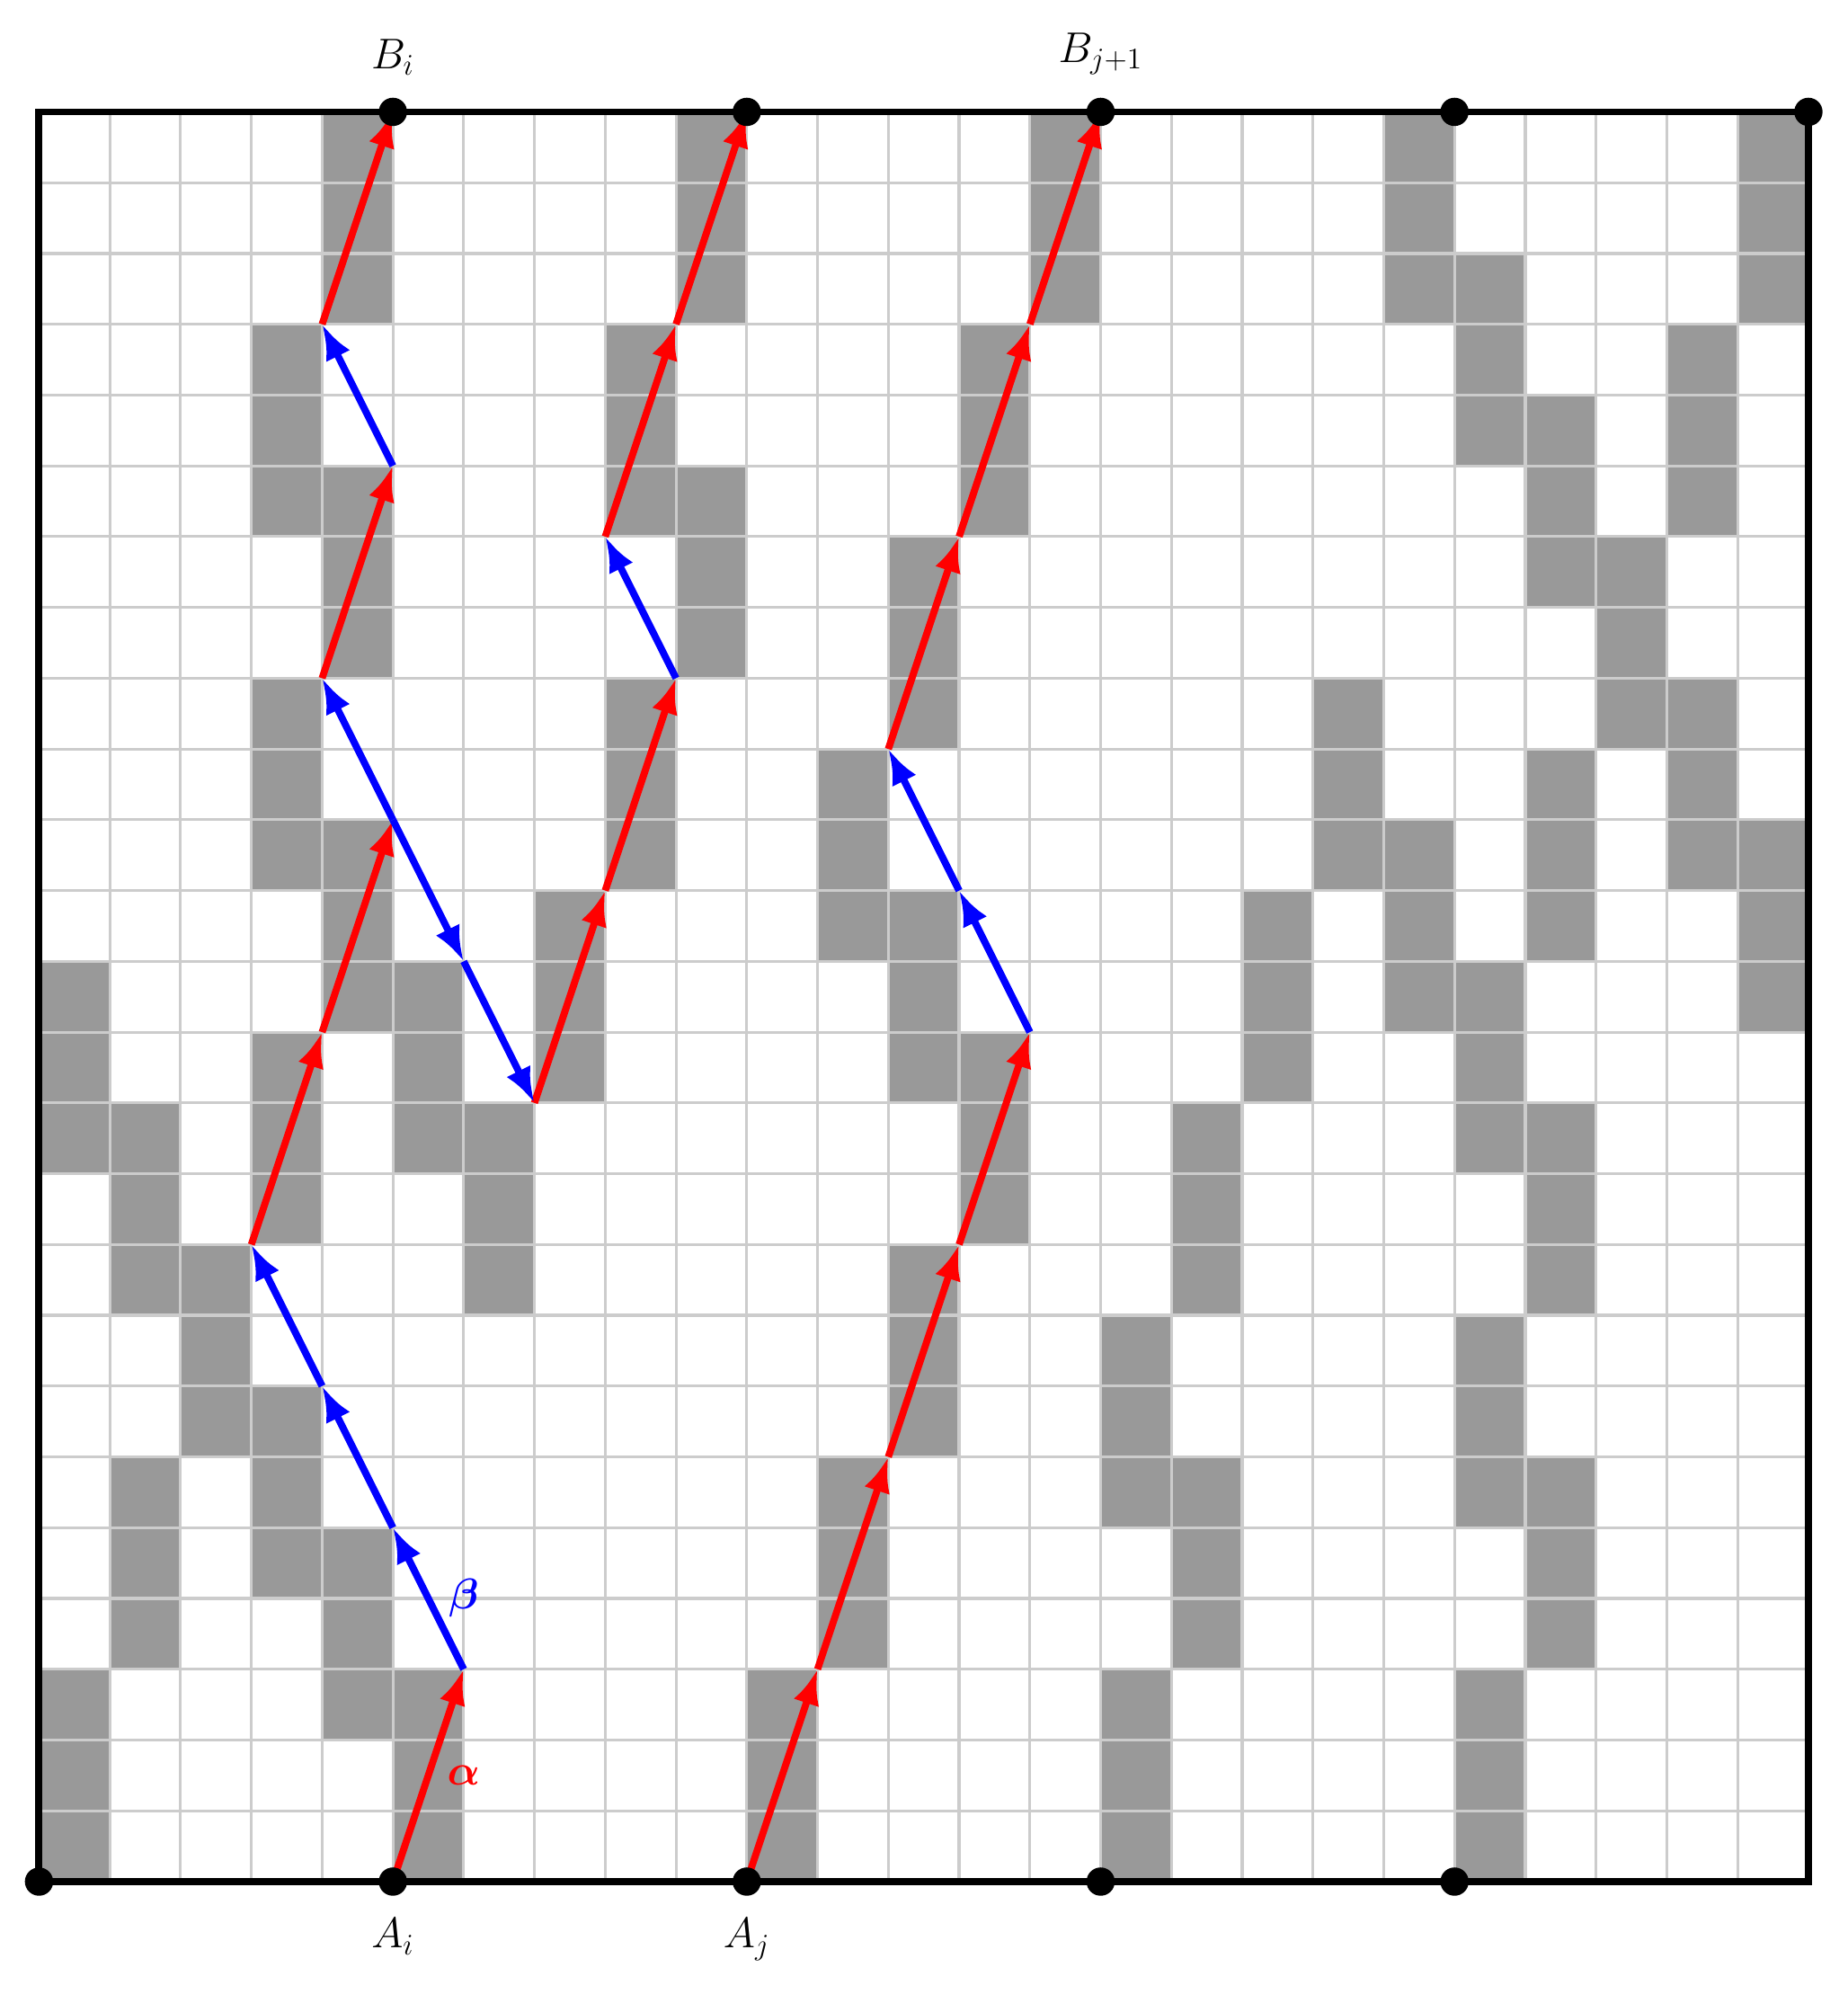
\begin{tikzpicture}
\foreach \a/\b in \D
    {\draw[black!40, line width=0.4mm, fill=black!40]
        (\a,\b) rectangle +(1,1)
        (\a,\b)++(0,1) rectangle +(1,1)
        (\a,\b)++(0,2) rectangle +(1,1);
	}
\draw[line width=0.4mm, black!20] (0,0) grid (25,25);
\draw[black, line width=1mm] (0,0)rectangle (25,25);
\foreach \a/\b in {5/0, 3/9, 4/12, 4/17, 4/22, 10/0, 11/3, 12/6, 13/9, 14/22, 12/16, 13/19, 7/11, 8/14, 8/19, 9/22}
    {\draw[red, line width=1mm, ->, >={Latex[length=5mm]}]
        (\a,\b) -- +(1,3);
	}
\foreach \a/\b in { 6/3 , 5/5 , 4/7, 5/15, 5/20, 14/12, 13/14, 9/17}
    {\draw[blue, line width=1mm, ->, >={Latex[length=5mm]}]
        (\a,\b) -- +(-1,2);
	}
\foreach \a/\b in {5/15 , 6/13}
    {\draw[blue, line width=1mm, ->, >={Latex[length=5mm]}]
        (\a,\b) -- +(1,-2);
	}
\node[below=0.4cm] at (5,0) {\LARGE$A_i$};
\node[above=0.4cm] at (5,25) {\LARGE$B_i$};
\node[below=0.4cm] at (10,0) {\LARGE$A_j$};
\node[above=0.4cm] at (15,25) {\LARGE$B_{j+1}$};
\node[red] at (6,1.5) {\LARGE$\bm{\alpha}$};
\node[blue] at (6,4) {\LARGE$\bm{\beta}$};
\fill[black] foreach \a in 
	{(0,0), (5,0), (10,0), (15,0), (20,0), 
	  (5,25), (10,25), (15,25), (20,25), (25,25)}
	{\a circle (2mm)};

\end{tikzpicture}
\end{document}